\documentclass[ngerman]{beamer}

\usepackage[utf8]{inputenc}
\usepackage[T1]{fontenc}
\usepackage{booktabs}
\usepackage{babel}
\usepackage{graphicx}
\usepackage{csquotes}
\usepackage{xcolor}
\usepackage{listings}
\usepackage{pdfpages}

\definecolor{hellgelb}{rgb}{1,1,0.8}
\definecolor{lightgelb}{rgb}{1,1,0.8}
\definecolor{colKeys}{rgb}{0,0,1}
\definecolor{colIdentifier}{rgb}{0,0,0}
\definecolor{colComments}{rgb}{1,0,0}
\definecolor{colString}{rgb}{0,0.5,0}

\usepackage{textcomp}
\lstset{%
	language=Python,%	
    float=hbp,%
    basicstyle=\ttfamily\footnotesize, %
    identifierstyle=\color{colIdentifier}, %
    keywordstyle=\color{colKeys}, %
    stringstyle=\color{colString}, %
    commentstyle=\color{colComments}, %
    alsoletter={\_},
	language= {Python},%
    columns=flexible, %
    tabsize=2, %
    morekeywords={read_csv,system,startfile,close,read,isoformat,now,to_datetime,merge,to_excel,join,concat,pairplot,vq,kmeans,savefig,Series,axis,DataFrame,index,to_frame,loc,iloc,idx,mean,describe,std,count,},%
    frame=single, %
    extendedchars=true, %
    showspaces=false, %
    showstringspaces=false, %
    numbers=left, %
    numberstyle=\tiny, %
    upquote=true,
    breaklines=true, %
    backgroundcolor=\color{yellow!15}, %
    breakautoindent=true, %
    captionpos=b%
}


\lstset{literate=%
    {Ö}{{\"O}}1
    {Ä}{{\"A}}1
    {Ü}{{\"U}}1
    {ß}{{\ss}}1
    {ü}{{\"u}}1
    {ä}{{\"a}}1
    {ö}{{\"o}}1
    {~}{{\textasciitilde}}1
}

\author{Uwe Ziegenhagen}
\title{Das \enquote{Köchelverzeichnis} von DANTE}
\subtitle{Die Bib\TeX-Datei aller DTK-Ausgaben}

\begin{document}

\begin{frame}

\maketitle

\end{frame}

\begin{frame}
\frametitle{Was ist das \enquote{Köchelverzeichnis}}
\framesubtitle{~}

Köchelverzeichnis

\begin{quote}
\enquote{Chronologisch-thematisches Verzeichniss sämmtlicher Tonwerke Wolfgang Amade Mozart’s. Nebst Angabe der verloren gegangenen, angefangenen, übertragenen, zweifelhaften und unterschobenen Compositionen desselben.}
\end{quote}

\begin{itemize}
	\item Erstellt von Ludwig Alois Friedrich Ritter von Köchel \newline (* 14.01.1800; † 03.06.1877)
	\item Erste Auflage des Verzeichnisses 1862
	\item War wohl nötig: \enquote{Sinfonie in D-Dur} beschrieb 20 Werke
	\item aktuell: 8. Auflage von 1964, wird gelegentlich nachgedruckt
	\end{itemize}


\end{frame}


\begin{frame}
\frametitle{Verbindung zu Dante e.V.}

Was hat das mit Dante e.V. zu tun?

\begin{itemize}
\item Liste meiner Publikationen für den Lebenslauf
\item Was habe ich eigentlich für die DTK geschrieben?
\item 440KB Bib-Datei vom DTK-Team, mit dem Hinweis der Unvollständigkeit
\end{itemize}
\end{frame}

\begin{frame}
\frametitle{JabRef Import}

\begin{center}
\fbox{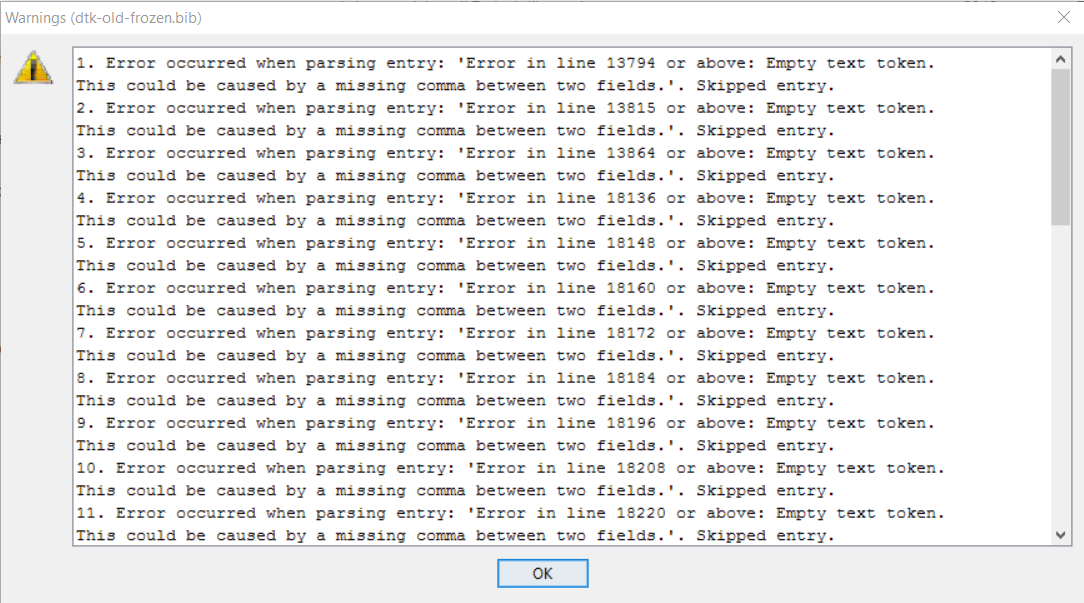
\includegraphics[width=\textwidth]{jabref-01}}
\end{center}
\end{frame}


\begin{frame}
\frametitle{JabRef Import}
\framesubtitle{~}

\begin{itemize}
	\item Letzter Eintrag aus dem Jahr 2013
	\item verschiedene andere Probleme\ldots
\end{itemize}

\begin{center}
\fbox{
\includegraphics[width=10cm]{jabref-02}}
\end{center}

\end{frame}

\begin{frame}
\frametitle{Aufarbeitung der Daten}

\begin{itemize}
\item \enquote{Progress is a slow process}
\item FrOSCon, Treffen mit Leo Arnold
\item Einrichtung GitHub Repository
\item \url{https://github.com/dante-ev/dtk-bibliography}
\item viel manuelle Arbeit vor allem durch Leo (Danke!)
\item \enquote{Interessante} Fehlersuche
\end{itemize}
\end{frame}

\begin{frame}
\frametitle{GitHub}

URL: \url{https://github.com/dante-ev/dtk-bibliography}

\begin{center}
\fbox{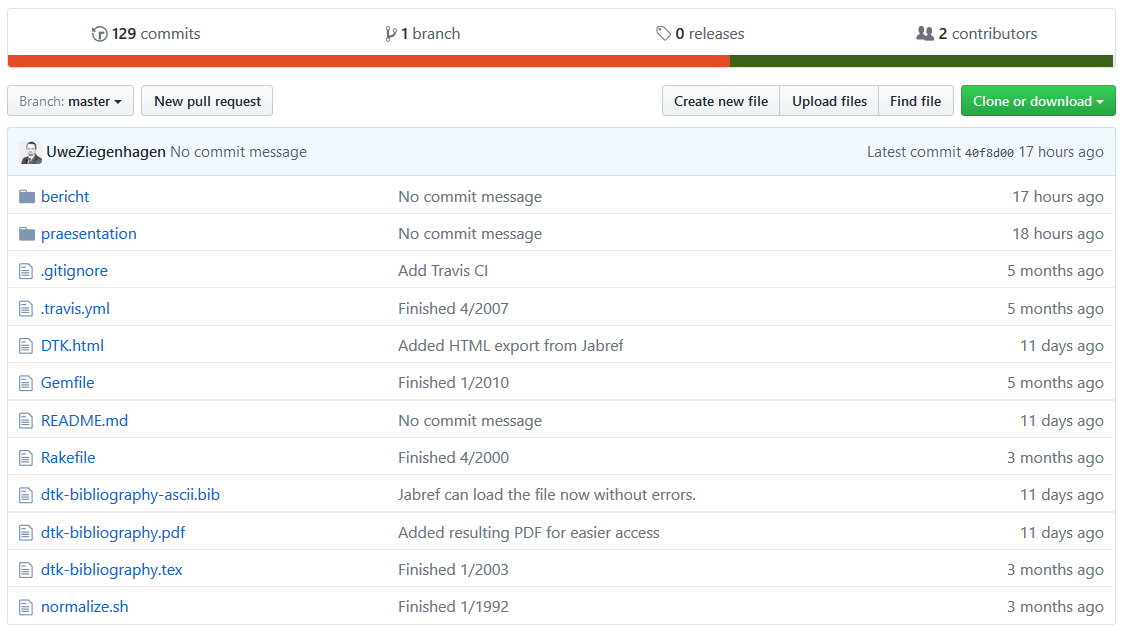
\includegraphics[width=\textwidth]{github-01}}
\end{center}
\end{frame}

\begin{frame}
\frametitle{GitHub}

\begin{itemize}
	\item Download/Clone ganz einfach
\end{itemize}

\begin{center}
\fbox{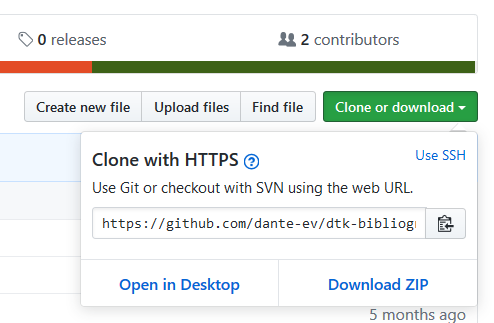
\includegraphics[width=\textwidth]{github-02}}
\end{center}
\end{frame}

\begin{frame}[fragile]
\frametitle{Reinigungsprozess}

\begin{center}
\fbox{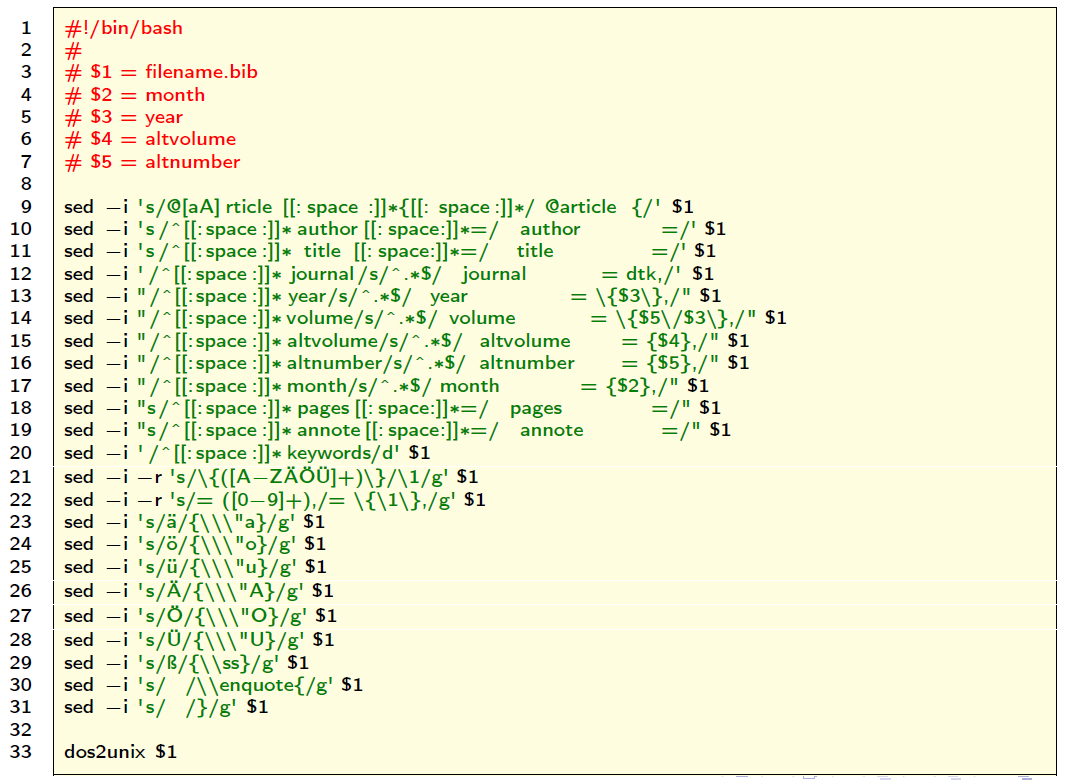
\includegraphics[width=0.95\textwidth]{normalize}}
\end{center}

\end{frame}


\begin{frame}
\frametitle{Reinigungsprozess}

\lstinputlisting[basicstyle=\scriptsize]{../Rakefile}

\end{frame}

\begin{frame}
\frametitle{Ergebnis}

\begin{itemize}
\item Alle DTKs seit 1989 sind bearbeitet, PDF-Datei von 57 Seiten (bei DIN A4)
\item Neue DTKs werden manuell hinzugefügt
\item Import in JabRef läuft fehlerfrei
\item Erlaubt Nutzung der JabRef Export-Filter
\item Zukünftig: Konsistenz-Checks, Datenqualität verbessern
\item Zusätzliche Versionen für z.B. Bib\LaTeX
\item Verlinkung zum PDF des einzelnen Artikels?
\end{itemize}
\end{frame}


\begin{frame}
\frametitle{Check Integrity\ldots}

\begin{center}
\fbox{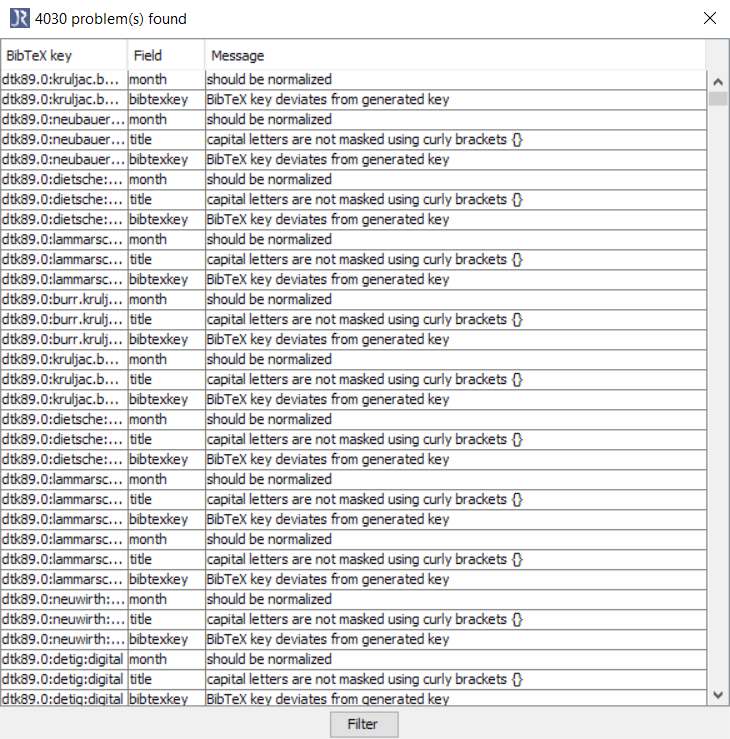
\includegraphics[width=0.7\textwidth]{normalized}}
\end{center}
\end{frame}



{
\setbeamercolor{background canvas}{bg=}
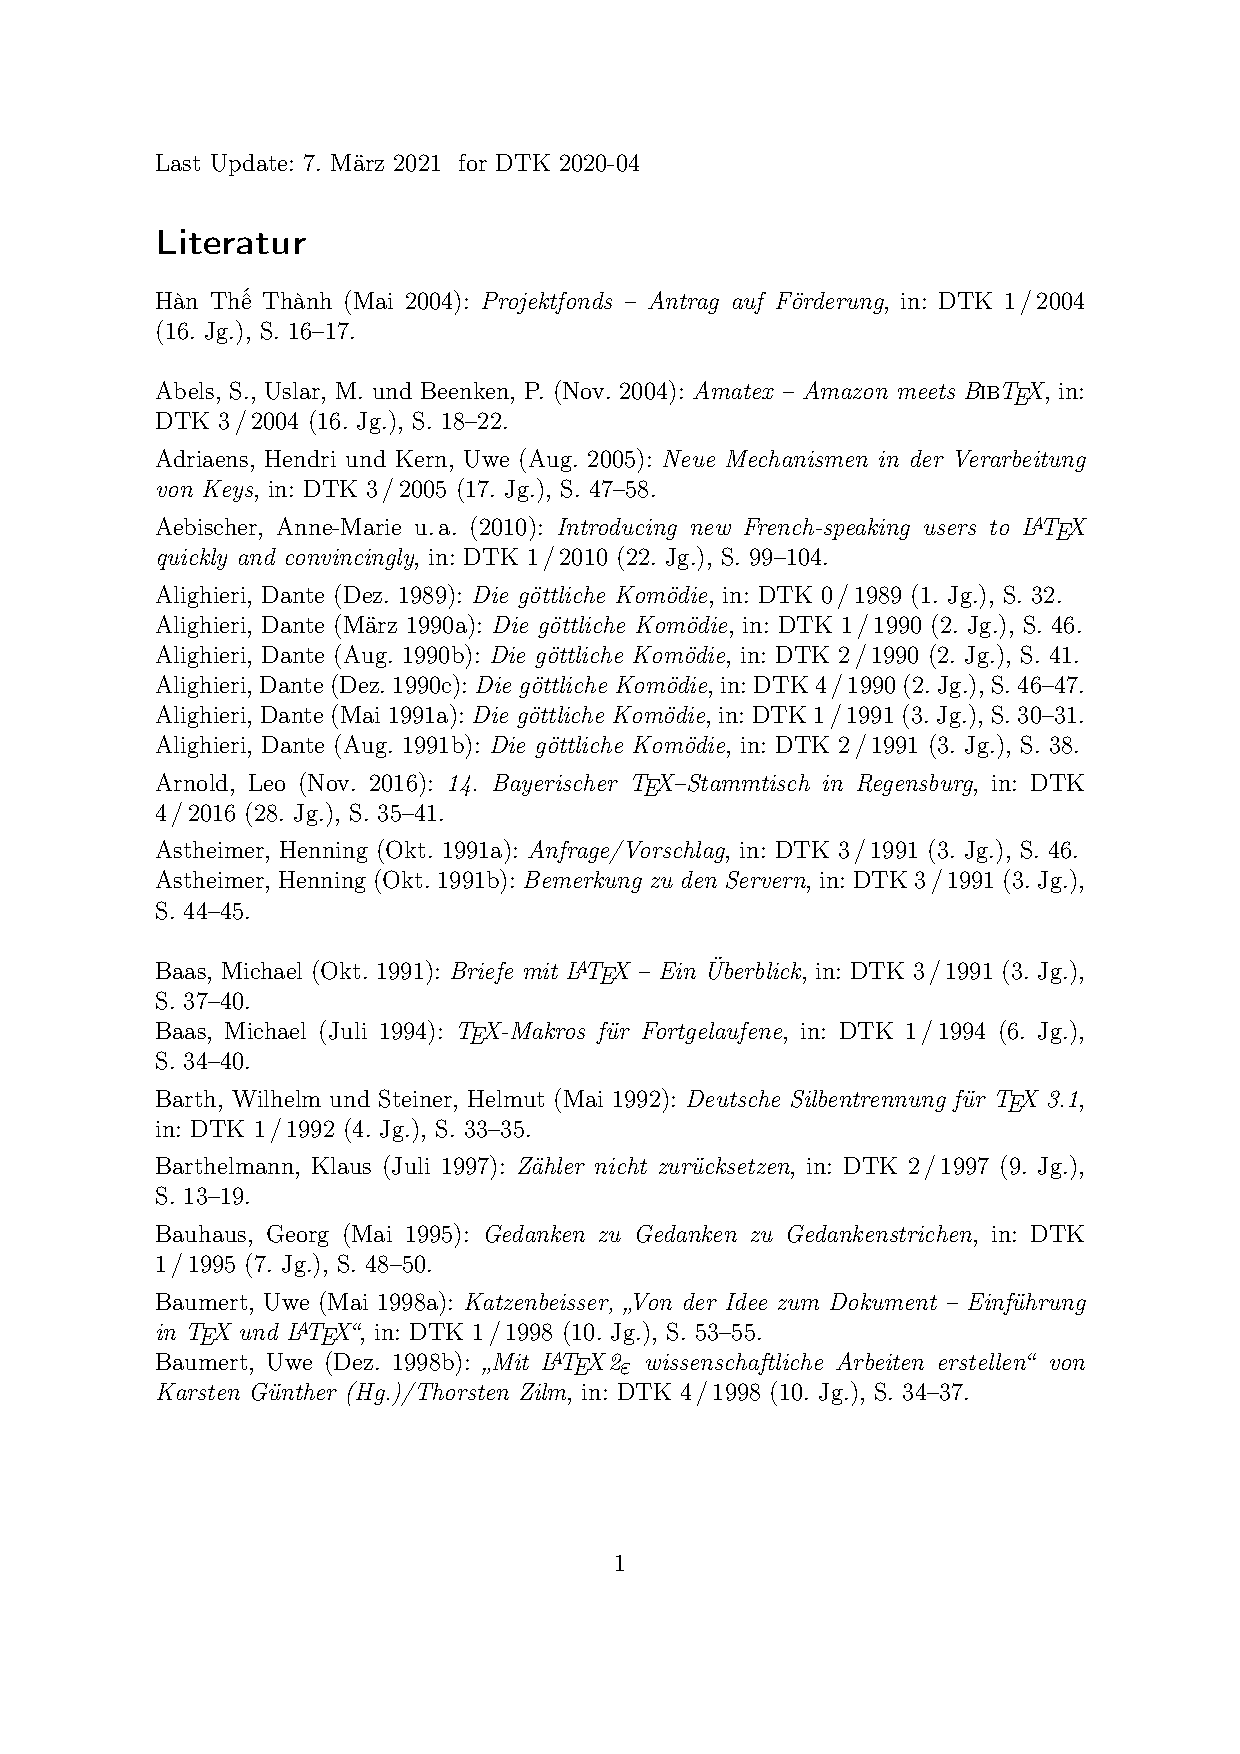
\includepdf[pages=1-191]{../dtk-bibliography.pdf}
}
\end{document}